\begin{figure}[!b]
\centering
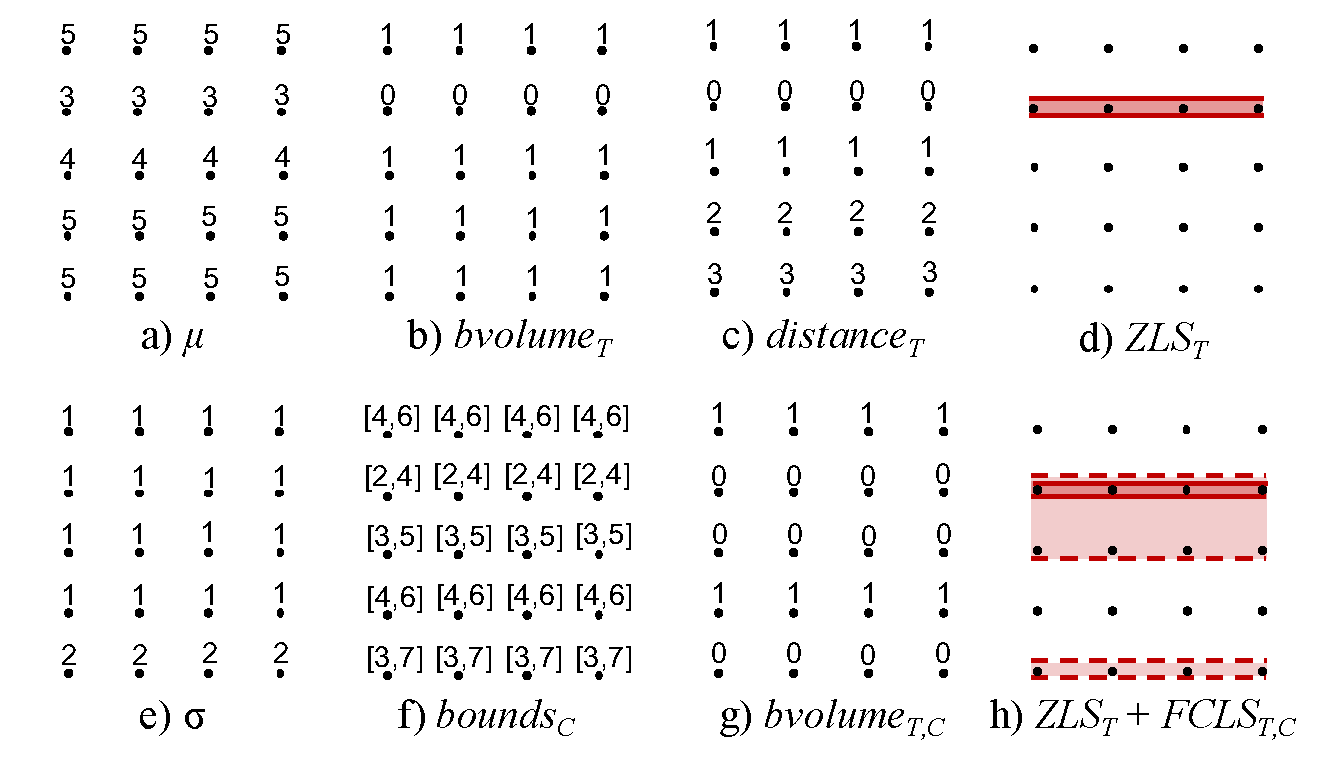
\includegraphics[width=\linewidth, trim={1cm 0cm 0.33cm 0cm}, clip]{Images/example_narrow.pdf}
%\vspace{-5mm}
\caption{A notional example showing the steps involved in generating the ``zero'' feature level-set $ZLS_{T}$~(top row) and feature confidence level-set $FCLS_{T,C}$~(bottom row) for an uncertain univariate field represented using ${\mu}$~(a) and ${\sigma}$~(e). 
%
For this example, we use trait $T=[2.5, 3.5]$ and confidence $C=68\%$, i.e., $Z=1$.
%
$FCLS_{T,C}$ is computed using the $distance_{T,C}$ (not shown) field.
%
Assuming a unit distance between adjacent grid points,
%
$distance_{T,C}$ would be computed using $bvolume_{T,C}$~(g) as input and would appear equivalent for this example.
%$bvolume_{T,C}$~(g) and $distance_{T,C}$ (not shown) would appear equivalent for this example.
}
%\vspace{-2mm}
\label{fig:example}
\end{figure}
